\lab{Python}{Data Structures}{Data Structures}
\label{lab:Python_DataStructures}
\objective{Empower students with basic knowledge of the fundamental, canonical data structures in order to understand performance and runtime characteristics.}

Both storing and retrieving data take time.
Whether its growth is logarithmic, linear, exponential, or factorial, as a data set grows, so too does the time it takes to manipulate it.
The overhead associated with working with large data sets makes it crucial that we have a fundamental knowledge of the data structures used to store them.
As we understand the characteristics of such data structures, we will be able to choose the data structure that will help us most efficiently access the data that we need.

\section*{Abstract Data Types}
The fundamental way to store data is via \emph{primitive data types}.
We are actually already quite familiar with these data types: booleans, strings, floats, and integers.
Most information that we care to store is in one of these forms; however, these primitive types can quickly become unwieldy for storing large amounts of information.
Imagine having a different name for every piece of data you use!
Luckily, we can create more natural ways to store data by using primitive data types, along with arrays, as our building blocks (consider object oriented programming).
More complex data structures are called \emph{abstract data types}.
Python possesses a couple of the more common abstract data types, including dictionaries and sets.
However, the performance of each abstract data type slows down as the size of the data structure increases.
 This is why it is so important that we understand the underlying advantages and disadvantages of these structures.

Most abstract data types use an object called a \emph{node} to store data.
A node essentially acts as a box in which we store an arbitrary piece of data.
What exactly \emph{is} a node, however?
A node is a building block for whichever kind of data structure we want to create: it is whatever we want it to be.
This versatility allows us to define nodes to store absolutely anything; what they contain both depends on the data structure itself and data that is actually being stored.
For example, the node of a binary search tree (which we will later discuss in section \ref{Binary Search Tree}) contains three things: a piece of data, a reference to its left child, and a reference to its right child.
The node of a linked list contains only two things: a piece of data and a reference to the next node it links to.

If we didn't use nodes, or ``data boxes'', we would have to build a new structure for each data type we wanted to store.
Thus, nodes allow us to abstract the data structure from the kind of data we store inside of them; nodes allow us to generalize the functionality of a data structure.

\section*{Linked Lists}
\emph{Linked lists} are one of the most basic of all abstract data structures.
A linked list, in essence, is simply a list of nodes that are linked together.
There are three common types of linked lists: singly-linked, doubly-linked, and circularly-linked.

\begin{figure}[h]
\centering
\begin{tikzpicture}[->,>=stealth',shorten >=1pt,auto, node distance=1.5cm,thick,main node/.style={rectangle,draw}, minimum size=.5cm]
\tikzset{rect node/.style={rectangle, draw, minimum height = .5cm, minimum width=.2cm}}
  \node[main node] (1) {B};
  \node[main node] (2) [right of=1] {F};
  \node[main node] (3) [right of=2] {G};
  \node[main node] (4) [right of=3] {C};
  \node[draw = none, black!20!blue, node distance=1.5cm] [above left of=1](H) {Head};
\foreach \r in {1, 2, 3, 4}{
  \node[rect node][right of=\r, node distance = .36cm]{};}
\node[draw = none, node distance = 1.5cm] [right of=4]{};  % Centralize this particular figure
\foreach \s/\t  in {1/2, 2/3, 3/4}{
	\path[draw](\s) edge[shorten <=.1cm](\t);}
  \draw[black!20!blue] (H) edge (1.north);
\end{tikzpicture}
\caption{Singly-linked List}
\end{figure}

A singly-linked node stores a piece of data (its value), and a single reference that points to the next node in the list.
We implement a singly-linked node class as follows:

\begin{lstlisting}
class Node():
    def __init__(self, data):
        self.next = None
        self.value = data
\end{lstlisting}

\begin{figure}[h]
\centering
\begin{tikzpicture}[->,>=stealth',shorten >=1pt,auto, node distance=1.5cm, thick,main node/.style={rectangle,draw}, minimum size=.5cm]
\tikzset{rect node/.style={rectangle, draw, minimum height = .5cm, minimum width=.9cm}}
  \node[main node] (1) {B};
  \node[main node] (2) [right of=1] {F};
  \node[main node] (3) [right of=2] {G};
  \node[main node] (4) [right of=3] {C};
  \node[draw = none, black!20!blue, node distance = 1.5cm] [above right of=4] (T) {Tail};
  \node[draw = none, black!20!blue, node distance = 1.5cm] [above left of=1] (H) {Head};
  \node[rect node](1.5)[]{};
  \node[rect node](2.5)[right of=1.5]{};
  \node[rect node](3.5)[right of=2.5]{};
  \node[rect node](4.5)[right of=3.5]{};

\foreach \s/\t  in {1/2, 2/3, 2/1, 3/2, 3/4, 4/3}{
	\path[draw](\s) edge[shorten <=.1cm, shorten >=.1cm](\t);}	
  \draw[black!20!blue] (H) edge (1.north);
  \draw[black!20!blue] (T) edge (4.north);
\end{tikzpicture}
\caption{Doubly-linked List}
\end{figure}

Doubly-linked nodes have two references: one that points to the previous node and one that points to the next node in the list.
This allows for a doubly-linked list to be traversed in both directions, whereas a singly-linked list can only be traversed in one direction.
We modify our node, then, to allow for a reference to the previous node.

\begin{lstlisting}
class Node():
    def __init__(self, data):
        self.next = None
        self.previous = None
        self.value = data
\end{lstlisting}

\begin{figure}[h]
\centering
\begin{tikzpicture}[->,>=stealth',shorten >=1pt,auto, node distance=1.5cm,
  thick,main node/.style={rectangle,draw}, minimum size=.5cm]
\tikzset{rect node/.style={rectangle, draw, minimum height = .5cm, minimum width=.2cm}}
  \node[main node] (1) {B};
  \node[main node] (2) [right of=1] {F};
  \node[main node] (3) [right of=2] {G};
  \node[main node] (4) [right of=3] {C};
  \node[](H) [above left of=1, node distance = 1.5cm, color = black!20!blue] {Head};
  \node[draw = none, black!20!blue, node distance = 1.5cm] [above right of=4] (T) {Tail};
  \node[rect node][right of=1, node distance = .36cm]{};
  \node[rect node][right of=2, node distance = .36cm]{};
  \node[rect node][right of=3, node distance = .36cm]{};
  \node[rect node](5)[right of=4, node distance = .36cm]{};
\foreach \s/\t  in {1/2, 2/3, 3/4}{
	\path[draw](\s) edge[shorten <=.1cm](\t);}
\path[] (5.east) edge[out=-70, in=-40] node[right] {} (1.south);
\path[black!20!blue]
    (H) edge (1.north)
    (T) edge (4.north);
\end{tikzpicture}
\caption{Circularly-linked List}
\end{figure}
A circularly-linked list is a special type of linked list (be it singly-linked or doubly-linked) where the last node (the \emph{tail}) of the list points to the first node (the \emph{head}) of the list as its next node.
In a circularly, doubly-linked list, the head also points to the tail as its previous node.

We begin constructing a singly-linked list class with a reference to the head node:
\begin{lstlisting}
class SLinkedList(object):
    def __init__(self):
        self.head = None
\end{lstlisting}

Linked lists may also have a reference to the tail node and a counter to keep track of the size of the list.
Including a tail reference allows us to avoid traversing the entire list each time we wish to insert at the end.
Similarly, without a counter we would have to recount the list every time we wanted to know its size.
\begin{lstlisting}
class SLinkedList(object):
    def __init__(self):
        self.head = None
        self.tail = None
        self.counter = 0

    def size(self):
        return self.counter
\end{lstlisting}

\subsection*{Finding, Inserting and Removing}
Unlike arrays, which have random access, a linked list must walk through each node, starting with its single reference to the head, to find later ones in the list.
In a singly-linked list, it is also often a good idea to track the node prior to our index; this will prove useful for our insertion and removal methods. 
We add a find method to our \li{SLinkedList} class:
\begin{lstlisting}
def find(self, index):
    nfind = self.head
    nprev = None
    count = 0
    if index >= self.counter:
        raise IndexError
    else:
        while count < index and nfind.next:
            count += 1
            nprev = nfind
            nfind = nfind.next
        return nprev, nfind
\end{lstlisting}

In order to insert or delete nodes found in the middle of the list, then, we must first locate the correct node by traversing the list - starting at the head and visiting each node.
Insertion itself is a very efficient procedure, but traversing the list to \emph{find} the insert location takes longer as the size of the list grows. 
However, because we already have head and tail references, nodes can be inserted or removed from either end of a linked list in \emph{constant time}.
This means the time a function takes is independent of the size of the list.
Methods that operate in constant time are key to understanding the advantages in efficiency of any particular data structure.

When we insert, we must remember to update the \li{next} reference in the node previous and to set the \li{next} reference in the new node we are inserting.
To insert into a linked list, we consider three cases: head insertion, tail insertion, and middle insertion. 

\begin{lstlisting}
    def insert(self, index, data):
        # Initialize a temporary node to store the desired piece of data.
        n = Node(data)        
        if index > self.counter:
            raise IndexError
        if index == 0: # Head insertion
            n.next = self.head
            # Set n as the new head node.
            self.head = n
            # If n is the only node, set as the tail.
            if self.counter == 0:
                self.tail = self.head
        elif index == self.counter: # Tail insertion
            self.tail.next = n
            # Set n as the new tail
            self.tail = n
        else: # Middle insertion
            nprev, nindex = self.find(index)
            n.next = nindex
            nprev.next = n
        self.counter += 1
\end{lstlisting}

\begin{problem}
Removing a node is similar to inserting a node, we must consider head removal, tail removal, and middle removal.
Implement a \li{remove(self, index)} method in your \li{SLinkedList} class.
Be sure to update your counter and references appropriately as you compensate for all possible situations  (the index corresponds to a list with a single node, the index is out of range, etc.)

The code below provides a few additional methods to supplement your \li{SLinkedList} class: one that will clear the list and one that will represent the list as a string.
These functions may be useful for testing your removal method.
\begin{lstlisting}
def clear(self):
    self.head = None

def __str__(self):
    return `[` + `,'.join(map(str, iter(self)) + `]'
    
def__iter__(self):
    temp = self.head
    while temp:
        yield temp.value
        temp = temp.right
\end{lstlisting}
\emph{Note}: Because Python is able to keep track of the variables we use, it will automatically delete a variable if there is no access to it.
In our \li{clear} method, this property allows us to set the reference to the head to be \li{None} which, in turn, allows Python to clean up the leftover nodes (in other languages, this might cause serious memory leaks).
\label{prob:LinkedList}
\end{problem}

\section*{Stacks, Queues, and Deques}
Stacks, queues (pronounced `cues'), and deques (pronounced `decks') can be thought of as types of linked lists where access is restricted.
Rather than accessing data anywhere in the list, we only add and remove from certain sides, which means that the methods of these structures operate in constant time.

\begin{itemize}
\item \emph{Stacks}: These are built on the in `last in, first out' principle, meaning that the last item that was put in the stack will be the first one to leave.
You can imagine this as a pile of plates in the kitchen cupboard.
Rarely, if ever, do you take the plate on the bottom of the pile.
Instead you take the one on the top.
When putting plates in the cupboard, you similarly put them on the top of the pile.
This means that the last plate put in will be the first one taken out.
To implement this, we would only add and remove from the same side of a linked list.
\item \emph{Queues}: Queues use a `first in, first out' implementation, meaning that the first thing put in will be the first thing taken out.
This is similar to people waiting in line.
The first person in line will be the first served and taken out of the line.
This is implemented as a linked list where we add on the right and remove from the left.
\item \emph{Deques}: This structure is a double-ended queue; we can add and remove from either end of a deque.
Really the only difference between this and a linked list is that we cannot add and remove from the middle.
Python's \li{collections} module already contains a deque object, which is discussed on page \pageref{deques} of our initial lab, \nameref{lab:Standard Library}.
\end{itemize}

\begin{problem}
Implement a queue and a stack by having them inherit from your linked list class.
Have your stack add to and remove from the right.
Have your queue add to the right and remove from the left.
\label{prob:Stack and queue}
\end{problem}

\section*{Trees}
\label{Binary Search Tree}
Donald Knuth, author of \emph{The Art of Computer Programming}, once said that ``Trees sprout up just about everywhere in computer science.''
\emph{Trees} are similar to linked lists, but the nodes of a tree can reference with greater versatility (rather than simply referencing the \li{next} and/or \li{previous} nodes).
Like the head node of a linked list, a tree begins with an initial reference node, here called the \emph{root} node.
Unlike linked lists, however, the nodes within a tree can point to multiple nodes (called \emph{child} nodes), depending on the way the tree is defined.
We can create many different types of trees by the way we organize the nodes within them; one of the simplest of these types is called a \emph{binary search tree} (BST).

A binary tree is a tree that has a maximum of two children per node, an ordered structure, and no duplicate elements.
Trees are commonly ordered such that the left half of the tree contains elements less than the root, and the right half contains elements greater than the root.
This type of organization substantially cuts down search time, making trees an excellent data structure to use when our primary goal is efficient searching.
By simply knowing that our target element is less or greater than the root, we can immediately eliminate half of our binary tree from the search.
Because the process of locating a node is so quick, the processes of inserting and removing nodes are similarly efficient.

We begin building a BST by defining our node class. A node in a binary search tree holds a piece of data as well as references to its left and right children (which can, in turn, be subtrees of this \emph{parent} node).
We call a node without any children a \emph{leaf} node.

\begin{lstlisting}
class Node(object):
    def __init__(self, data):
        self.value = data
        self.left = None
        self.right = None
\end{lstlisting}
We initialize our BST similarly to a linked list, with a reference to the root and to a counter to keep track of the size.
\begin{lstlisting}
class BinTree(object):
    def __init__(self):
        self.root = None
        self.size = 0
\end{lstlisting}

\subsection*{Inserting}
Inserting a node into a binary search tree is a simple procedure.
Our goal is to insert into a leaf node, so we recursively insert to the right if the element is greater than the current node or insert to the left if the element is less than the current node.
Once we reach a node without a left or right subtree, we add our new node as its new child node.
Thus, we always insert into leaf nodes; we never insert a non-leaf node into a BST.

Let's demonstrate this process with an example.

\begin{minipage}{0.35\textwidth}
    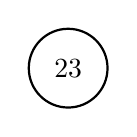
\begin{tikzpicture}[thick]
      \node[circle, draw, minimum size = 1cm]{23};
    \end{tikzpicture}
\end{minipage}\hfill
\begin{minipage}{0.55\textwidth}
    We start with an empty tree, and add our root node: $23$.
\end{minipage}

\begin{minipage}{0.35\textwidth}
    \begin{tikzpicture}[
      node distance = 1.5cm,
      level distance=1.5 cm,
      level 1/.style={sibling distance=3cm},
      level 2/.style={sibling distance=1.5cm},
      thick, minimum size=1cm]
      \node[circle,draw](23) {23}
	    child {
	    node [circle,draw](17){17}
	    }
	    child{node[circle,draw](476){476}
	    };
      \path[->, >=stealth', shorten >=1pt, auto]
	    (23) edge[bend right, blue] (17)
	    (23) edge[bend left, red] (476);
    \end{tikzpicture}
\end{minipage}\hfill
\begin{minipage}{0.55\textwidth}
    Now we add two children: $17$ and $476$.
    Clearly, $17$ becomes the left child because $17 < 23$, and $476$ becomes the right child because $476 > 23$.
\end{minipage}

\begin{minipage}{0.35\textwidth}
    \begin{tikzpicture}[
      node distance = 1.5cm,
      level distance=1.5 cm,
      level 1/.style={sibling distance=3cm},
      level 2/.style={sibling distance=1.5cm},
      thick, minimum size=1cm]
      \node[circle,draw] {23}
	    child {
	    node [circle,draw]{17}
	    }
	    child{node[circle,draw]{476}
		    child{node[circle,draw](28){28}}
		    child[fill=none] {edge from parent[draw=none]}
	    };
      \path[->, >=stealth', shorten >=1pt, auto]
      (23) edge[bend left, red] (476)
      (476) edge [bend right, blue] (28);
    \end{tikzpicture}
\end{minipage}\hfill
\begin{minipage}{0.55\textwidth}
    What happens if we add $28$? Starting at the root, we move to the right because $28 > 23$.
    However, there is already a right subroot there!
    $28$ must then take $476$ as its parent node and, because $28 < 476$, it is placed as the left child of $476$.
\end{minipage}

To begin writing an insertion method for our \li{BinTree} class, we consider BST's themselves.
BSTs are a recursive data structure because each of the left and right subtrees of a parent node are, themselves, BSTs.
Therefore, many of the algorithms for working with binary search trees are also recursive.
A recursive function is a function that calls itself until it reaches a base case.
To supplement our \li{insert} method, we write a recursive function to call within our insert function:
\begin{lstlisting}
def insert(self, data):
    def _recur_insert(node, item):
        # This base case identifies the proper leaf node for
        # insertion and returns the data as a Node.
        if node is None:
            return Node(item)
        # Allows you to recursively travel through the binary tree
        # until you reach a leaf node.
        else:
            if data < node.value:
                node.left = _recur_insert(node.left, item)
            elif data > node.value:
                node.right = _recur_insert(node.right, item)
        # After the base case, each of the previous calls to
        # the recursive function finish by returning the previous node.
        return node
    self.root = _recur_insert(self.root, data)
    self.size += 1
\end{lstlisting}
We call this recursive function by setting it equal to the root node.
The function will continually call itself until it finds an empty node, insert the data as a \li{Node()}, and use \li{return node} to finish each of the previous calls to the recursive function. 
(It simply returns each of the parents it recursively visited prior, re-setting them equal to themselves, until it finally returns to \li{self.root}.)
Finally, we finish our insertion method by updating our counter.

\subsection*{Finding}
Although recursive functions are often useful and intuitive with trees, we  are by no means required to use them.
In fact, for large trees, a recursive algorithm will consume a lot of resources.
When writing a method to search for nodes in a BST, we may either use recursion or an alternate method to ascertain whether a piece of data is, indeed, to be found within the tree.

\begin{problem}
Add a method for finding nodes to your binary tree class. If a node containing your data exists within the tree, return the node.
If no such node exists, return \li{False}.
\label{Finding Nodes}
\end{problem}

\subsection*{Removing}
Removing nodes is only slightly more complicated.
We have three cases to consider:
\begin{enumerate}
\item No children.
This is the most straightforward case.
If the node we want to delete has no children then we simply remove the node.
\begin{center}
\begin{minipage}{0.3\textwidth}
    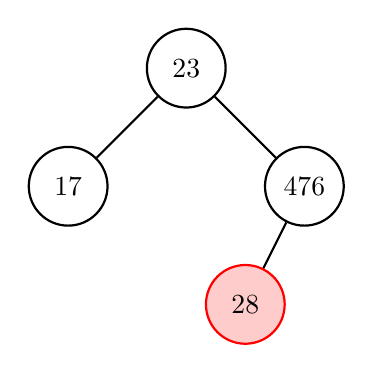
\begin{tikzpicture}[
      level distance=1.5 cm,
      level 1/.style={sibling distance=3cm},
      level 2/.style={sibling distance=1.5cm},
      thick, minimum size=1cm]
      \node[circle,draw](23) {23}
	    child {
	    node [circle,draw](17){17}
	    }
	    child{node[circle,draw](476){476}
	    	child{node[circle,draw=red, fill=red!20!](28){28}}
	    	child[fill=none] {edge from parent[draw=none]}
	    };
    \end{tikzpicture}
\end{minipage}
\begin{minipage}{0.2\textwidth}
   \begin{center}
     \begin{tikzpicture}[]
        \draw[->, double, double equal sign distance, -implies, thick] (0,0) -- (1.25,0);
    \end{tikzpicture}
   \end{center}
\end{minipage}
\begin{minipage}{0.3\textwidth}
    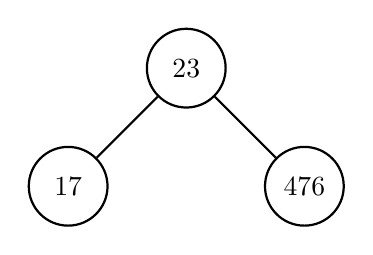
\begin{tikzpicture}[
      level distance=1.5 cm,
      level 1/.style={sibling distance=3cm},
      level 2/.style={sibling distance=1.5cm},
      thick, minimum size=1cm]
      \node[circle,draw](23) {23}
	    child {
	    node [circle,draw](17){17}
	    }
	    child{node[circle,draw](476){476}
	    };
    \end{tikzpicture}
\end{minipage}
\end{center}

\item One child.
In this case, we have to worry about children.
If we were to just delete the node, we would lose the entire subtree.
The solution, however, is simple enough: we promote the single child to take the place of the node we are deleting.
\begin{center}
\begin{minipage}{0.3\textwidth}
    \begin{tikzpicture}[
      level distance=1.5 cm,
      level 1/.style={sibling distance=3cm},
      level 2/.style={sibling distance=1.5cm},
      thick, minimum size=1cm]
      \node[circle,draw](23) {23}
	    child {
	    node [circle,draw](17){17}
	    }
	    child{node[circle,draw=red, fill = red!20!](476){476}
	    	child{node[circle,draw](28){28}}
	    	child[fill=none] {edge from parent[draw=none]}
	    };
     \path[->, >=stealth', shorten >=1pt, auto]
      (28) edge[bend left, red] (476);
    \end{tikzpicture}
\end{minipage}
\begin{minipage}{0.2\textwidth}
   \begin{center}
     \begin{tikzpicture}[]
        \draw[->, double, double equal sign distance, -implies, thick] (0,0) -- (1.25,0);
    \end{tikzpicture}
   \end{center}
\end{minipage}
\begin{minipage}{0.3\textwidth}
    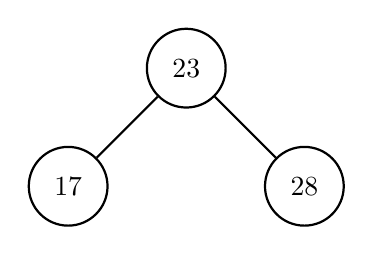
\begin{tikzpicture}[
      level distance=1.5 cm,
      level 1/.style={sibling distance=3cm},
      level 2/.style={sibling distance=1.5cm},
      thick, minimum size=1cm]
      \node[circle,draw](23) {23}
	    child {
	    node [circle,draw](17){17}
	    }
	    child{node[circle,draw](28){28}
	    };
    \end{tikzpicture}
\end{minipage}
\end{center}
\item Two children.
We need to be a little careful in this case.
We can't simply promote a child node.
Indeed, how would we decide which child to promote?
Fortunately, we can reduce this case down to one of the previous two cases.
Suppose we are removing node $23$, which has two children.
We first locate the \emph{in order successor}: either the smallest node of the right subtree or the greatest node of the left subtree.
In this case, we identify node $28$ as the in order successor.
Note that, because $28$ is the smallest node of the right subtree, it cannot have a child to it's left, which implies it either has one child to the right or no children at all.
We swap the data of nodes $28$ and $23$ (so node $28$ now has the data that $23$ had and vice versa).
Thus, removing $23$ has been reduced to a simpler case.
\begin{center}
\begin{minipage}{0.3\textwidth}
\begin{tikzpicture}[
  level distance=1.5 cm,
  level 1/.style={sibling distance=3cm},
  level 2/.style={sibling distance=1.5cm},
  thick, minimum size=1cm]
  \node[circle,draw=red, fill = red!20!](23) {23}
	child {
	node [circle,draw]{17}
	}
	child{node[circle,draw]{476}
		child{node[circle,draw](28){28}}
		child[fill=none] {edge from parent[draw=none]}
	};	
  \node[draw=none, node distance=3cm](Note)[right of =28] {In order successor};
  \path[->, >=stealth', auto]
     (Note) edge (28)
     (23) edge[out = 5, in=15, blue, looseness=1.5] (28)
     (28) edge[bend left, red] (23);
\end{tikzpicture}
\end{minipage}
\begin{minipage}{0.2\textwidth}
   \begin{center}
     \begin{tikzpicture}[]
        \draw[->, double, double equal sign distance, -implies, thick] (0,0) -- (1.25,0);
    \end{tikzpicture}
   \end{center}
\end{minipage}
\begin{minipage}{0.3\textwidth}
    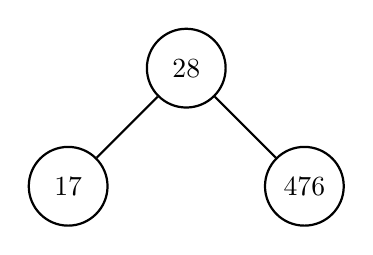
\begin{tikzpicture}[
      level distance=1.5 cm,
      level 1/.style={sibling distance=3cm},
      level 2/.style={sibling distance=1.5cm},
      thick, minimum size=1cm]
      \node[circle,draw](28) {28}
	    child {
	    node [circle,draw](17){17}
	    }
	    child{node[circle,draw](476){476}
	    };
    \end{tikzpicture}
\end{minipage}
\end{center}
\end{enumerate}

\begin{problem}
Give your binary tree class a method for removing nodes.
Make sure to account for each of the three cases presented above.

\emph{Helpful Hint}: It may be a good idea to write a recursive function to call within your remove method. 
\label{prob:Binary Removal}
\end{problem}

\subsection*{Balanced Trees}
Binary search trees often perform very well if the primary goal for our structure is efficient searching.
However, the order of insertion into a binary search tree largely determines how well the tree performs.
Binary search trees work best when elements are added in a random order.
This keeps the levels of the tree relatively complete, rather than imbalanced where certain subtrees are far larger than others.
If the elements are sorted before they are added to a BST, the efficiency of using a binary search tree is completely mitigated.
As is evident in figure \ref{fig:Degenerate Tree}, the resulting degenerate tree is essentially a linked list.
\begin{figure}[h]
\centering
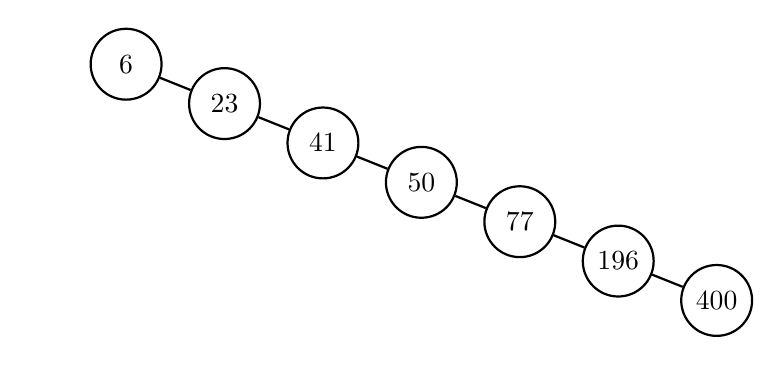
\begin{tikzpicture}[
  level distance=.5 cm, % level and sibling distance edited to allow for the tree to fit on the page, and to better resemble a linked list
  level 1/.style={sibling distance=2.5cm},
  level 2/.style={sibling distance=2.5cm},
 thick, minimum size = .9cm]
    \node[circle,draw] {6}
	child[fill=none] {edge from parent[draw=none]}	
	child {node[circle,draw]{23}
		child[fill=none] {edge from parent[draw=none]}
		child{node[circle,draw]{41}
			child[fill=none] {edge from parent[draw=none]}
			child{node[circle,draw]{50}
				child[fill=none] {edge from parent[draw=none]}
				child{node[circle,draw]{77}
					child[fill=none] {edge from parent[draw=none]}
					child{node[circle,draw]{196}
						child[fill=none] {edge from parent[draw=none]}
						child{node[circle,draw]{400}}
					}
				}
			}
		}
	};
\end{tikzpicture}
\caption{Example of a degenerate tree}
\label{fig:Degenerate Tree}
\end{figure}

One method for solving these problems is to keep the tree balanced.
On each insertion and removal, the tree is re-balanced to maintain optimal performance.
AVL trees (Adelson-Velskii and Landis' Trees) and red-black trees are examples of balanced trees.
Figure \ref{fig:AVL btree} displays the elements from figure \ref{fig:Degenerate Tree} as an AVL-balanced tree.
\begin{figure}[h]
\centering
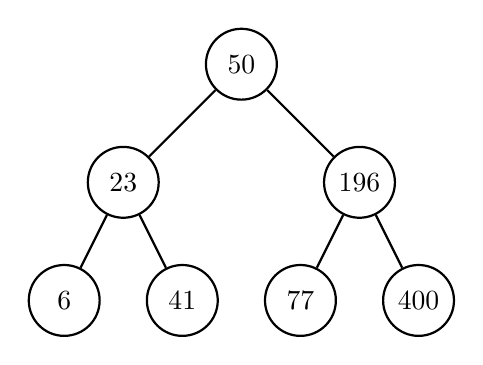
\begin{tikzpicture}[
  level distance=1.5 cm,
  level 1/.style={sibling distance=3cm},
  level 2/.style={sibling distance=1.5cm},
 thick, minimum size = .9cm]
  \node[circle,draw] {50}
	child {node[circle,draw]{23}
		child{node[circle,draw]{6}
		}
		child{node[circle,draw]{41}
		}
	}
	child{node[circle,draw]{196}
		child{node[circle,draw]{77}
		}
		child{node[circle,draw]{400}
		}
	};
\end{tikzpicture}
\caption{Example of an AVL-balanced tree}
\label{fig:AVL btree}
\end{figure}

We will not discourse upon the specific algorithms for AVL balancing or red-black balancing here.
However, a comparison between the two figures makes it clear that a balanced tree will enable far more efficient searching than an unbalanced tree.

\section*{Heaps}
A \emph{heap} is another tree-based data structure; however, heaps are only partially ordered and are always \emph{complete}.
In a complete tree, every level of the tree, except possibly the last, is filled to its capacity.
Furthermore, each of the leaves on the last level of a complete tree must be oriented to the left.
Heaps are always complete because of the way they are partially ordered: parents are ordered with respect to children, but unlike a BST, siblings or cousins have no order.
In a max heap, for example, each parent is greater than its children.
However, the order of the children within each level doesn't matter, as long as each child is less than its parent node.
\begin{figure}[h]
\begin{centering}
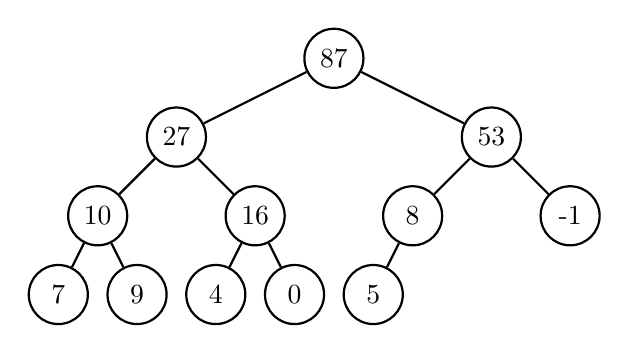
\begin{tikzpicture}[
  level distance=1 cm, % Normally, this distance would be 1.5cm, but the original pictures to imitate are more condensed
  level 1/.style={sibling distance=4cm}, % Adjust the level distance to compensate for additional nodes
  level 2/.style={sibling distance=2cm},
  level 3/.style={sibling distance=1cm},
  minimum size = .75cm, thick]
  \node[circle,draw](87) {87}
	child {node[circle,draw]{27}
		child{node[circle,draw]{10}
			child{node[circle,draw]{7}}
			child{node[circle,draw]{9}}
		}
		child{node[circle,draw]{16}
			child{node[circle,draw]{4}}
			child{node[circle,draw]{0}}
		}
	}
	child{node[circle,draw]{53}
		child{node[circle,draw]{8}
			child{node[circle,draw]{5}}
			child[fill=none] {edge from parent[draw=none]}
		}
		child{node[circle,draw]{-1}}
	};
\end{tikzpicture}
\end{centering}
\caption{Example of a max heap}
\label{fig:Max Heap}
\end{figure}
Note, as in figure \ref{fig:Max Heap}, that this ordering puts the maximum of the heap at the root of the tree.
Therefore, the partial ordering of a heap makes finding the root very efficient; we often use max or min heaps when we need to find the maximum or minimum of a data set in constant time.
We are also commonly use heaps for \emph{priority queues}, because the only element we need access to is the one with the greatest priority.
However, because heaps are only partially ordered, searching for nodes in heap, other than the root, is not as efficient a procedure as in a BST.

To add into a heap, we put the node into the farthest left available leaf on the lowest level of the tree.
Then we compare it to its parent according to our chosen ordering: in the max heap below, if the node is greater than its parent, we switch the two nodes.
We continue this process until either the new node reaches a greater parent or until it becomes the new root.

\begin{minipage}{.65\textwidth}

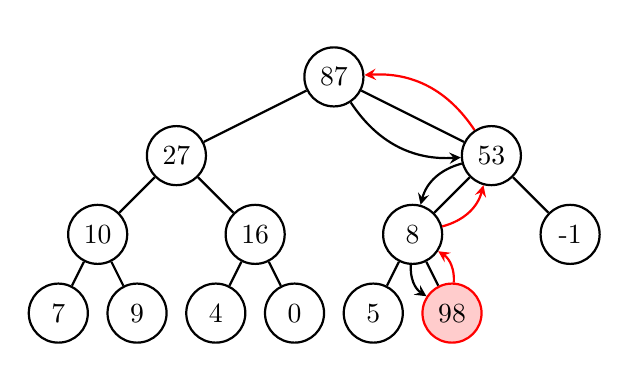
\begin{tikzpicture}[
  level distance=1 cm, % Normally, this distance would be 1.5cm, but the original pictures to imitate are more condensed
  level 1/.style={sibling distance=4cm}, % Adjust the level distance to compensate for additional nodes
  level 2/.style={sibling distance=2cm},
  level 3/.style={sibling distance=1cm},
  minimum size = .75cm, thick]
  \node[circle,draw](87){87}
	child {node[circle,draw]{27}
		child{node[circle,draw]{10}
			child{node[circle,draw]{7}}
			child{node[circle,draw]{9}}
		}
		child{node[circle,draw]{16}
			child{node[circle,draw]{4}}
			child{node[circle,draw]{0}}
		}
	}
	child{node[circle,draw](53){53}
		child{node[circle,draw](8){8}
			child{node[circle,draw]{5}}
			child{node[circle,draw=red, fill=red!20!](98){98}}
		}
		child{node[circle,draw]{-1}
        }
	};
\foreach \s/\t in {98/8, 8/53, 53/87}{
    \path[->, >=stealth, auto]
	    (\s) edge[bend right, red] (\t)
        (\t) edge[bend right] (\s);}
\node[draw=none, node distance = .25cm][above of=87]{};
\end{tikzpicture}
\begin{tikzpicture}[
  level distance=1 cm, % Normally, this distance would be 1.5cm, but the original pictures to imitate are more condensed
  level 1/.style={sibling distance=4cm}, % Adjust the level distance to compensate for additional nodes
  level 2/.style={sibling distance=2cm},
  level 3/.style={sibling distance=1cm},
  minimum size = .75cm, thick]
  \node[circle,draw](98){98}
	child {node[circle,draw]{27}
		child{node[circle,draw]{10}
			child{node[circle,draw]{7}}
			child{node[circle,draw]{9}}
		}
		child{node[circle,draw]{16}
			child{node[circle,draw]{4}}
			child{node[circle,draw]{0}}
		}
	}
	child{node[circle,draw]{87}
		child{node[circle,draw]{53}
			child{node[circle,draw]{5}}
			child{node[circle,draw]{8}}
		}
		child{node[circle,draw]{-1}
        }
	};
\node[draw=none, node distance = 3.25cm][below of=98]{};
\draw[->, double, double equal sign distance, -implies, thick, shorten >=.2cm, shorten <=.2cm]
        (0,1.5) -- (0,.5);
\end{tikzpicture}
\end{minipage}
\begin{minipage}{.3\textwidth}
In the example to the left, we add element $98$ to our Max heap.
We begin by inserting $98$ as the next available leaf on the bottom level.
Now we must compare it to its parent, $8$.
Because $98 > 8$, the two nodes switch locations on the heap.
This pattern continues with each successive parent-child comparison: $98 > 53$, and $98 > 87$.
Finally, our inserted node, $98$, becomes the new root (and therefore the new maximum) of this heap.
\end{minipage}

Since heaps are really only useful for keeping track of the root, removing the maximum is easy, but removing any other node is not.
To remove the maximum (the root), we simply compare the root's children and promote the greatest to be the new root.

\section*{Hash Tables}
A \emph{hash table} is a very simple data structure that trades space for speed.
The key advantage of a hash table is this speed; most of the operations of a hash table execute in constant time, independent of the size of the data structure.
Unlike previous data structures we have studied, however, we do not construct a hash table by defining a node class.
In essence, a hash table is actually an array where each piece of data is associated with its index as a key.
As such, hash tables have very fast lookup times; they form the underlying data structure of Python's dictionaries.

One of the key components of a hash table is a \emph{hash function}.
A hash function takes our data as an input and then outputs a positive integer used to index the array.
Since the hash function must be executed to perform any operation on the hash table, it is important that the hash function executes quickly.
Thus, the heart of a hash table is a good hash function.

We begin defining our \li{HashTable} class, then, by allocating space within a one-dimensional array (a Python list) and by taking both the array size and the hash function as arguments.
\begin{lstlisting}
class HashTable(object):
    def __init__(self, hsize, hashfunc):
        # Efficiently extends a list to the designated hash table size.
        self.hashtable = [None] * hsize
        # Keeps track of the number of elements within the hash table.
        self.elsize = 0
        # Indicates the size of the hash table
        self.hsize = hsize
        # Indicates the hash function
        self._hash = hashfunc
\end{lstlisting}

What makes a good hash function?
Hash functions need to distribute items evenly throughout the hash table.
Since we usually mod by the table size at the end (to keep the index within proper range), we need to make sure the remainders mod $n$ are evenly distributed.
Consider a simple example where we use a hash table to store strings.
Our hash function will index a string by the string's length mod the size of the table.
As the size of such a hash table grows, however,  fewer and fewer strings will be hashed to its end: the function won't distribute the data evenly.
Therefore, before we mod the string length by the table size, we multiply by a large prime number.
A large number helps guarantee that the remainders will vary, and the prime helps prevent us from multiplying by a multiple of the table size (which would send us to $0$ every time).
\begin{lstlisting}
def HashFunction(string, tablesize, prime=5417):
    index = (len(string) * prime)  %  Tablesize
    return index
\end{lstlisting}
Let's apply our example hash function to a table of size 4.
Then `cat' would be stored at index $3$ and `lion' would be stored at index $0$.
\begin{center}
\begin{tikzpicture}[thick]
\tikzstyle{block} = [rectangle, draw, minimum height = .55cm, minimum width = 1.5cm]
    \node[block] (0) [] {`lion'};
    \node[block] (1) [right=-.03 cm of 0] {}; % The -.03 ensures that our table lines intersect, rather than combine to create thicker lines.
    \node[block] (2) [right=-.03 cm of 1] {};
    \node[block] (3) [right=-.03 cm of 2] {`cat'};
\tikzstyle{block} = [draw=none]
\foreach \s in {0, 1, 2, 3}{
    \node[block] [above=0cm of \s]{\s};}
\end{tikzpicture}
\end{center}
\begin{problem}
Add an insert method to your \li{HashTable} class. Don't forget to update your counter for the number of elements within the hashtable!

Initialize a hash table of size 11 using the example \li{HashFunction()} from above.
Add the following felines: `lion', `tiger', `cheetah', `cougar', `colocolo', and `cat'.
Print your hash table. What happens when you insert `clouded leopard'?
What happens when you insert `jaguar'?
\label{Prob:Basic hash insert}
\end{problem}

As we saw in the previous problem, our example hash function is still far from perfect.
In our example hash table, if we try to store the string `leopard', our hash function sends it to 3.
But `cat' is already stored in spot 3!
This is called a \emph{hash collision}.
So how can we deal with collisions?
\begin{center}
\begin{tikzpicture}[->,>=stealth',shorten >=1pt, auto,thick]
\tikzstyle{block} = [rectangle, draw, minimum height = .55cm, minimum width = 1.5cm]
   \node[block] (0) [] {`lion'};
   \node[block] (1) [right=-.03 cm of 0] {};
   \node[block] (2) [right=-.03 cm of 1] {};
   \node[block] (3) [right=-.03 cm of 2] {`cat'};
\tikzstyle{block} = [draw=none]
\foreach \s in {0, 1, 2, 3}{
    \node[block] [above=0cm of \s]{\s};}
   \node[block, node distance = 1.5cm, red] (leopard) [below right of=3]{`leopard'};
   \path[red]
   (leopard.west) edge[bend left] (3.south);
   \node[draw = none, node distance = 1.75cm] [left of=0]{};  % Centralize this particular figure
\end{tikzpicture}
\end{center}

The ideal hash function maps unique inputs to unique outputs that are uniformly distributed over the hash space.
However, it is extremely difficult to create an ideal hash function; most hash functions will experience hash collisions.
Fortunately, there are ways to handle hash collisions.
The two methods that we will discuss are called open addressing and chaining.

\subsection*{Open Addressing}
The term \emph{open addressing} indicates that the output of the hash function doesn't necessarily identify the location of the piece of data.
\emph{Probing} is one of the more popular forms of open addressing; in this section we will discuss both linear and quadratic probing.

In the event of a hash collision, linear probing seeks to resolve the collision by looking for the next available location in the hash table.
We can do this by sequentially visiting each location and, when we find an empty one, storing our data in that location.
The following is an example of a linear probing hash function where $n$ is the size of the hash table, $h(x)$ is the hash function, and $i$ is a constant:
\begin{equation*}
h(x, i) = h(x) + i \pmod{n}
\end{equation*}

We start with $i = 0$, and if the spot is full, we increment $i$ until we find an empty spot.
If we go back to our earlier example, we can store `leopard' in our hash table using linear probing.
Our hash function sends us to spot 3, but it is already filled, so we start stepping through the table.
Since 3 is at the end of the table, we go to the beginning (namely $4 \% 4$) and, because spot 0 is already filled, we proceed to index 1.
Spot 1 is empty, so we store `leopard' there.
\begin{center}
  \begin{tikzpicture}[->,>=stealth',shorten >=1pt, auto, thick]
 \tikzstyle{block} = [rectangle, draw, minimum height = .55cm, minimum width = 1.5cm]
   \node[block] (0) [] {`lion'};
   \node[block] (1) [right=-.03 cm of 0] {`leopard'};
   \node[block] (2) [right=-.03 cm of 1] {};
   \node[block] (3) [right=-.03 cm of 2] {`cat'};
\tikzstyle{block} = [draw=none]
\foreach \s in {0, 1, 2, 3}{
    \node[block] [above=0cm of \s]{\s};}
   \node[block, node distance = 1.5cm, red] (leopard) [below right of=3]{`leopard'};
   \path[red]
   (leopard.west) edge[bend left] (3.south)
   (3.south) edge[bend left] (0.south)
   (0.south) edge[bend right, out=-20, shorten <=.2cm] (1.south);
  \end{tikzpicture}
\end{center}
\begin{problem}
Expand the \li{insert} method of your \li{HashTable} class to enable linear probing.
Do not allow your method to insert, however, if the hash table is full.
From your previous hash table, again add `clouded leopard' and `jaguar'.
Which index does your new insert method send `clouded leopard' to?
What about `jaguar'?
\label{prob:Linear probing insert}
\end{problem}

When we use linear probing to insert a piece of data, how can we later find it?
If we simply use our hash function, we will be directed to the incorrect index.
We then have to begin iterating through the table to search for our data.
Let's supplement our \li{HashTable} class with a \li{find} method.
\begin{lstlisting}
def find(self, data):
    index = self._hash(data, self.hsize)
    # Steps through the table until it reaches either the data or 
    # the initial index.
    for i in xrange(self.hsize):
        newindex = (index + i) % self.hsize
        # Optional step: prints the indices each step of the search.
        print 'Searching ' + str(newindex)
        if self.hashtable[newindex] == data:
            return True
    return False
\end{lstlisting}

Though linear probing is certainly a valid method to resolve hash collisions, it has its own set of drawbacks.
For example, a linear probe tends to cause elements in the table to cluster together.
Furthermore, if our hash table is densely populated or our hash function has a lot of collisions, we lose the efficiency of a hash table because we must resort to a linear search.
Quadratic probing seeks to mitigate the issues associated with linear probing by spreading out hash collisions more evenly.
A quadratic probing hash function where $c_1$ and $c_2$ are constants is of the form
\begin{equation*}
h(x, i) = h(x) + c_1i + c_2i^2 \pmod{n}
\end{equation*}

\subsection*{Chaining}
Chaining is a form of \emph{closed addressing}, meaning that the output of the hash function actually does point to the location of the data.
With chaining, each location of the hash table references a list of the data pieces sent to that index.
When one or more pieces of information hash to the same location, they are simply appended to that location's list.

Let's add `leopard' to our earlier example, this time using chaining.
Our hash function sends us to 3, but `cat' is already there.
Thus we add `leopard' to the list in spot 3 that already contains `cat'.
\begin{center}
\begin{tikzpicture}[->,>=stealth',shorten >=1pt, auto, thick]
 \tikzstyle{block} = [rectangle, draw, minimum height = .55cm, minimum width = 1.5cm]
    \node[block] (0) [] {`lion'};
    \node[block] (1) [right=-.03 cm of 0] {};
    \node[block] (2) [right=-.03 cm of 1] {};
    \node[block] (3) [right=-.03 cm of 2] {`cat'};
    \node[block, node distance = 1.5cm](leopard)[below of=3]{`leopard'};
\tikzstyle{block} = [draw=none]
\foreach \s in {0, 1, 2, 3}{
    \node[block] [above=0cm of \s]{\s};}
   \draw[->] (3) -- (leopard);
\end{tikzpicture}
\end{center}

\begin{problem}
Improve your \li{insert} method to deal with hash collisions via chaining, rather than probing. 
Note that, with this method, you need not return an error if the hash table is already full (the new insertion will simply be appended to the proper index's list).
Recreate and print your feline hash table(including 'jaguar' and 'clouded leopard') using this new method of insertion. 
\label{prob:Chaining insert}
\end{problem}

With a good hash function, the average size of the hash location's list is relatively short, so searching the list doesn't affect the overall performance of the hash table.
We update our \li{find} method to search a hash table implemented via chaining:
\begin{lstlisting}
def find(self, data):
    index = self._hash(data, self.hsize)
    for i in self.hashtable[index]:
        if i == data:
            return True
    return False
\end{lstlisting}

\subsection*{Hash Table Details}
As a hash table fills up, its performance degrades.
This is because more hash collisions occur, forcing us to use either linear probing or chaining to resolve them.
As a result, we have to search through lists or iterate through the table more often.
To combat this, we often track a \emph{load factor} for the hash table.
This load factor reveals how `saturated' the table is by calculating the ratio of the number of elements in the hash table to the size of the hash table.
We can easily add method to calculate the load factor of our \li{HashTable} class:
\begin{lstlisting}
def load(self):
    loadfactor = float(self.elsize)/self.hsize
    return loadfactor
\end{lstlisting}

When the load factor exceeds a certain threshold, we must allocate more space for the table.
However, since the hash function was dependant on the size of the table, we need to re-hash everything already in the table.
This can sometimes be a very expensive operation.
It's important to avoid resizing the table whenever possible.

After adding `leopard' into our earlier example, our hash table is very full. Let's re-hash it into a table with size 8.
Our new hash function sends a string to its size mod 8 (rather than mod 4, as before).
`cat' is sent to 3, `lion' to 4, and `leopard' to 7.
Now that we have no hash collisions, there are no lists to iterate through and our hash table performs far more efficiently.
\begin{center}
\begin{tikzpicture}[->,>=stealth',shorten >=1pt, auto, thick]
 \tikzstyle{block} = [rectangle, draw, minimum height = .55cm, minimum width = 1.5cm]
    \node[block] (0) [] {};
\foreach \s/\t/\u in {1/0/ , 2/1/ , 3/2/ , 4/3/`cat', 5/4/`lion', 6/5/ , 7/6/`leopard'}{
    \node[block] (\s) [right=-.03 of \t] {\u};}
\tikzstyle{block} = [draw=none]
\foreach \s in {0, 1, 2, 3, 4, 5, 6, 7}{
    \node[block] [above=0cm of \s]{\s};}
\end{tikzpicture}
\end{center}

\begin{problem}
Create a method for your hash table to resize.
Implement this method such that, if the load factor exceeds $.75$, it will resize the hash table so that the load factor will be below $.33$.
Don't forget to rehash the elements already within the table.
Call this resize method at the end of your insertion method, so that the function never inserts into a saturated table.

Now, insert `siberian tiger' and `bengal tiger' into your feline hash table. What is its new size? 
\label{prob:Hash resizing}
\end{problem}
\begin{comment}
\section*{Sparse Matrices}
Matrices are powerful tools, but they can take a lot of space in memory.
A $n \times n$ matrix takes $n^2$ places of storage!
If every entry in the matrix is useful information this is fine, but if the matrix is filled with a lot of zeros, that means we are using almost $n^2$ spots in memory to store useless zeros.
Not only does this unnecessarily take up space, it means that during computation we will spend a lot of time adding and multiplying zeros.
That can be a lot of useless computation.
The solution to this is \emph{sparse matrices}.
They are other data structures used to represent a matrix by only storing non-zero entries.

One common way is a dictionary.
The index of the spot in the matrix is the key and the number in that spot is the value.
For example,
\[
\begin{pmatrix}
0 & 0 & 0 & 0 & 0 \\
22 & 0 & 0 & 0 & 0 \\
0 & 0 & 0 & 0 & 0 \\
0 & 0 & 5 & 0 & 0 \\
0 & 0 & 0 & 0 & -4
\end{pmatrix}
\]
would be stored as
\[
\begin{tabular}{|c|l|}
\hline
Key & Value \\
\hline
(1,0) & 22 \\
\hline
(3,2) & 5 \\
\hline
(4,4) & -4 \\
\hline
\end{tabular}
\].

In this case, we stored a 5 by 5 matrix in a dictionary with only 3 key-value pairs.

SciPy has a nice implementation of sparse matrices.
Not only does SciPy reduce the amount of space needed to store matrices, it has fast algorithms for matrix operations that takes advantage of the fact that there are so many zeros.

\begin{problem}
Use your time function from Section 1 and the code given below to time matrix multiplication using sparse matrices versus normal matrix multiplication for $ n = 100, 500, 1000, 1500,$ and $2000$. Which is faster? What happens as the matrices grow larger?
\begin{lstlisting}
from scipy import sparse
import numpy as np

#dimension of matrices
n = 100

# create 2 random sparse matrices with density 0.1
A = sparse.rand(n,n)
B = sparse.rand(n,n)

#Multiply using sparse matrix techniques
A.dot(B)

#Change to dense matrices
A_dense = A.todense()
B_dense = B.todense()

#Multiply with normal matrix multiplication
A_dense.dot(B_dense)

 \end{lstlisting}
 \label{prob:Sparse}
 \end{problem}
\end{comment}


